\documentclass[aspectratio=169]{beamer}

%
% Choose how your presentation looks.
%
% For more themes, color themes and font themes, see:
% http://deic.uab.es/~iblanes/beamer_gallery/index_by_theme.html
%
\mode<presentation>
\mode<presentation>
{
  \usetheme{Ilmenau}      % or try Darmstadt, Madrid, Warsaw, ...
  \usecolortheme{beaver} % or try albatross, beaver, crane, ...
  \usefonttheme{default}  % or try serif, structurebold, ...
  \setbeamertemplate{navigation symbols}{}
  \setbeamertemplate{caption}[numbered]
  \useoutertheme{smoothbars}
  \setbeamercolor{section in head/foot}{bg=red!60!black}
  \setbeamercolor{section in head/foot}{fg=white!90!black}
 
  
} 
\usepackage[english]{babel}
\usepackage[utf8x]{inputenc}
\usepackage{graphicx,adjustbox}
\usepackage{setspace}
\usepackage{tikz} \usetikzlibrary{snakes}
\usepackage{epstopdf}
\usepackage[round]{natbib}
\setbeamertemplate{enumerate items}[circle]
\setbeamertemplate{itemize items}[circle]
\setbeamertemplate{blocks}[rounded][shadow=false] 
\usepackage{remreset}% tiny package containing just the \@removefromreset command
\makeatletter
\@removefromreset{subsection}{section}
\makeatother
\setcounter{subsection}{1}
\setbeamertemplate{section in toc}[sections numbered]


\newcommand*\oldmacro{}%Pages at the bottom right corner
\let\oldmacro\insertshorttitle%
\renewcommand*\insertshorttitle{%
	\oldmacro\hfill%
	\insertframenumber\,}


\usepackage[english]{babel}
\usepackage[utf8x]{inputenc}
\title[Local Housing Markets]{Housing Bubbles and Incumbent Support}
\author[Larsen et al.]{Martin Vinæs Larsen \qquad Frederik Hjorth \qquad Peter Thisted  Dinesen  \and  \\ Kim Mannemar  Sønderskov \vspace{0.1in}  \\Departments of Political Science \\ Aarhus University \\ University of Copenhagen \ }
\date[Sept. 2nd 2016]{New Directions in Policy Feedback Research \\ American Political Science Association Annual Meeting \\ September 2nd 2016}


\begin{document}
	
	\begin{frame}
		\titlepage
	\end{frame}
	
	\begin{frame}
		\tableofcontents

	\end{frame}
	
	
		\AtBeginSection[]{\begin{frame}
				\tableofcontents[currentsection] 
			\end{frame}}
			

\section{Local housing markets}
\begin{frame}
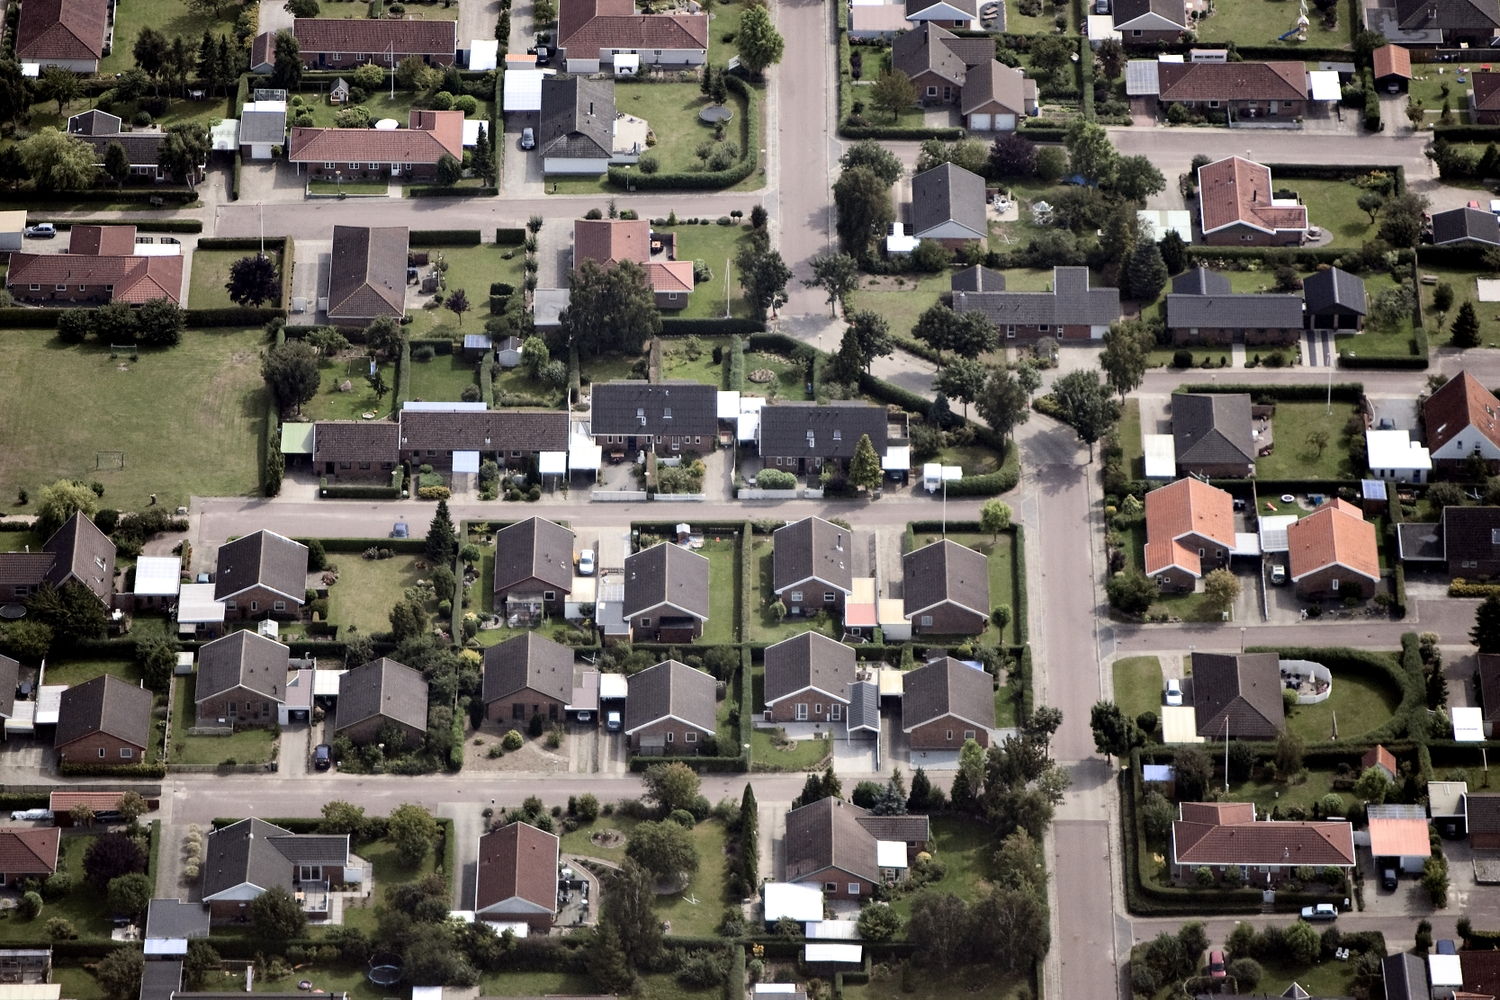
\includegraphics[width=1\textwidth]{../../figures/villakvarter.jpg}
\end{frame}

\begin{frame}
Important part of the economy: Local housing markets.

\vspace{0.1in} \pause

We saw this in the great recession, which was kick-started by a housing bubble.  \pause

\vspace{0.1in}
\begin{figure} \centering

\includegraphics[width=0.2\textwidth]{../../figures/99homes.jpg} \hspace{0.2in} \pause 
\includegraphics[width=0.4\textwidth]{../../figures/bigshort.jpg}
\end{figure}
\vspace{0.1in}
\pause	
	
Potential political effects? 
  \pause
$\rightsquigarrow$ Local housing prices drive incumbent support.
\end{frame}

\begin{frame}
Voters infer smth about quality of economic management from local housing prices. \pause

	
$\rightsquigarrow$ type of rational retrospective voting

\vspace{0.2in} \pause
	
Motive might be geo-, ego- or sociotropic. \pause

$\rightsquigarrow$ we are not going to be able to distinguish between  different motives. \pause
\vspace{0.2in}
	
Important: We look at support for incumbent, not preferences for redistribution.  	
\end{frame}


\section{The Danish Case}
\begin{frame}
Our case is Denmark ca. 2002 - 2015.\pause

\begin{enumerate}[<+->]
	\item In this period DK experienced very volatile housing bubble.
	\item The housing bubble was largely driven by policies instated by gov't in 2002/3.
	\item Detailed data from the national registers on local housing markets in this period.
	\item We link the housing market data to voting behavior in two different ways.
\begin{itemize}[<+->]
	\item Precinct-level election returns
	\item Two-wave panel survey of reported voting
\end{itemize}
\end{enumerate}

\end{frame}

\section{Precinct-level data}

\begin{frame}
DV is support for gov't parties at precincts across elections in '05, '07, '11, '15.

$\rightsquigarrow$  smallest unit at which election outcomes are observed ($3,000$ voters on average)

\vspace{0.2in} \pause
IV is year-over-year changes in the price of real-estate sold in the precinct's zip code.

$\rightsquigarrow$ Data from the Danish Mortgage Federation. \pause

\vspace{0.2in}

We link precincts to zip-codes by identifying the zip code of the precinct's polling place.

$\rightsquigarrow$  we also have information on unemployment and median income in each zip-code.
 

	
\end{frame}

\begin{frame} 
\begin{center}	
	\huge{ \noindent $govt_{it}=$  $\Delta price_{it} $ \only<1>{$+ \epsilon_{it}$} \pause $+ \gamma_t$ \only<2>{$+ \epsilon_{it}$} \pause $+ \pi_i$ \only<3>{$+ \epsilon_{it}$} \pause  $+ econ \beta$ \only<4->{$+ \epsilon_{it}$} \pause

\vspace{0.2in}
\noindent $govt_{it-1}=$  $\Delta price_{it} $ $+ \gamma_t$ $+ \pi_i$  $+ econ \beta$ $+ \epsilon_{it}$
}
\end{center}
\end{frame}



\begin{frame} \centering
		\foreach \n in {1,2,3,4,5,6}{
	
	\includegraphics<\n>[width=0.8\textwidth]{../../figures/lagd\n.eps}
}
\end{frame}




\section{Individual-level data}

\begin{frame}
We also test the proposition using a two-wave panel survey of Danish citizens.

$\rightsquigarrow$ Interviewed at different points of time in the aughts, re-interviewed in '11. \pause


$\rightsquigarrow$ Link these respondents to the national registers.

\vspace{0.1in} \pause
	
Why use this data as well?
\begin{itemize} \pause
	\item Replication (/methodological triangulation). \pause
	\item Explore individual level moderators to get at mechanism. \pause
	\item Allows us to define context in flexible ways (cf. MAUP).
\end{itemize}
\end{frame}


\begin{frame} 
	\centering

\foreach \n in {1,2,3,4,5,6}{\noindent \begin{adjustbox}{max width=0.5\textwidth} \only<\n>{\input{../../figures/illustrate\n.txt} } \end{adjustbox}}	 
\end{frame}



\begin{frame} 
	DV is reported vote choice for gov't party. \pause
	
	\vspace{0.2in} 
	IV is changes in the price of real-estate sold in residential context (dif interpretations).
	\vspace{0.2in}  \pause
	
	We use a linear regr with fixed effects to estimate the effect of local housing prices. \pause
	
	$\rightsquigarrow$ Controls: Unemployment, Income (personal, context) \pause
	
	$\rightsquigarrow$ Use an LPM as a link function. 
	
	
\end{frame}

\begin{frame} \centering
	\foreach \n in {1,2,3,4,5,6,7}{
		
		\includegraphics<\n>[width=0.8\textwidth]{../../figures/comparison\n.eps}
	}
	
	%Not significant
\end{frame}

\begin{frame} \centering
	\foreach \n in {1,2,3,4,5,6,7}{
		
		\includegraphics<\n>[width=1\textwidth]{../../figures/moderator\n.eps}
	}
	
	%Not significant
\end{frame}
\section{Conclusion}

\begin{frame}
We find that local housing prices do drive incumbent support. \pause

$\rightsquigarrow$ especially for those who engage with the local housing market. \pause

\vspace{0.2in}
Suggests that local economy matters. \pause
\begin{itemize}[<+->]
	\item People make inferences about pol's based on how local community is doing.
	\item Means that pol's need to worry about `geography of grievances'.
\end{itemize}

\vspace{0.2in} \pause
Also suggests that, more broadly, housing markets matter politically.

$\rightsquigarrow$ voters will adapt, focus on new parts of the economy. 
\end{frame}

\end{document}